\documentclass[aspectratio=169,10pt]{beamer}
\usetheme{Madrid}
\usepackage[T1]{fontenc}
\usepackage{lmodern}
\usepackage{tikz}
\usepackage{adjustbox}
\usepackage{array}
\usetikzlibrary{shapes.geometric,arrows.meta,positioning,calc,fit,backgrounds}

% Brand Color Palette matching PrismSpace theme
\definecolor{prismNavy}{RGB}{13,29,54}
\definecolor{prismBlue}{RGB}{38,126,190}
\definecolor{prismTeal}{RGB}{28,161,157}
\definecolor{prismMint}{RGB}{232,248,245}
\definecolor{prismGold}{RGB}{229,166,50}
\definecolor{prismDark}{RGB}{15,23,42}
\definecolor{prismIndigo}{RGB}{79,70,229}
\definecolor{prismSlate}{RGB}{71,85,105}
\definecolor{cardBg}{RGB}{248,250,252}

\setbeamercolor{frametitle}{bg=prismNavy,fg=white}
\setbeamertemplate{navigation symbols}{}
\setbeamertemplate{footline}{\hfill\textbf{PrismSpace} $\cdot$ CSE, CEK\hspace{1em}|\hspace{1em}\insertframenumber/\inserttotalframenumber\hspace{1.5em}\vspace{0.4em}}

\newcommand{\pk}[1]{\textbf{#1}}
\newcommand{\idx}[1]{\textit{#1}}
\newcommand{\comp}[1]{\texttt{#1}}

\begin{document}

\begin{frame}[t]{04. Browser Database Schema: \texttt{PrismDB} (Figure 4.4)}
\vspace{-0.35cm}
\centering
\adjustbox{max width=0.98\linewidth, max height=0.85\textheight}{%
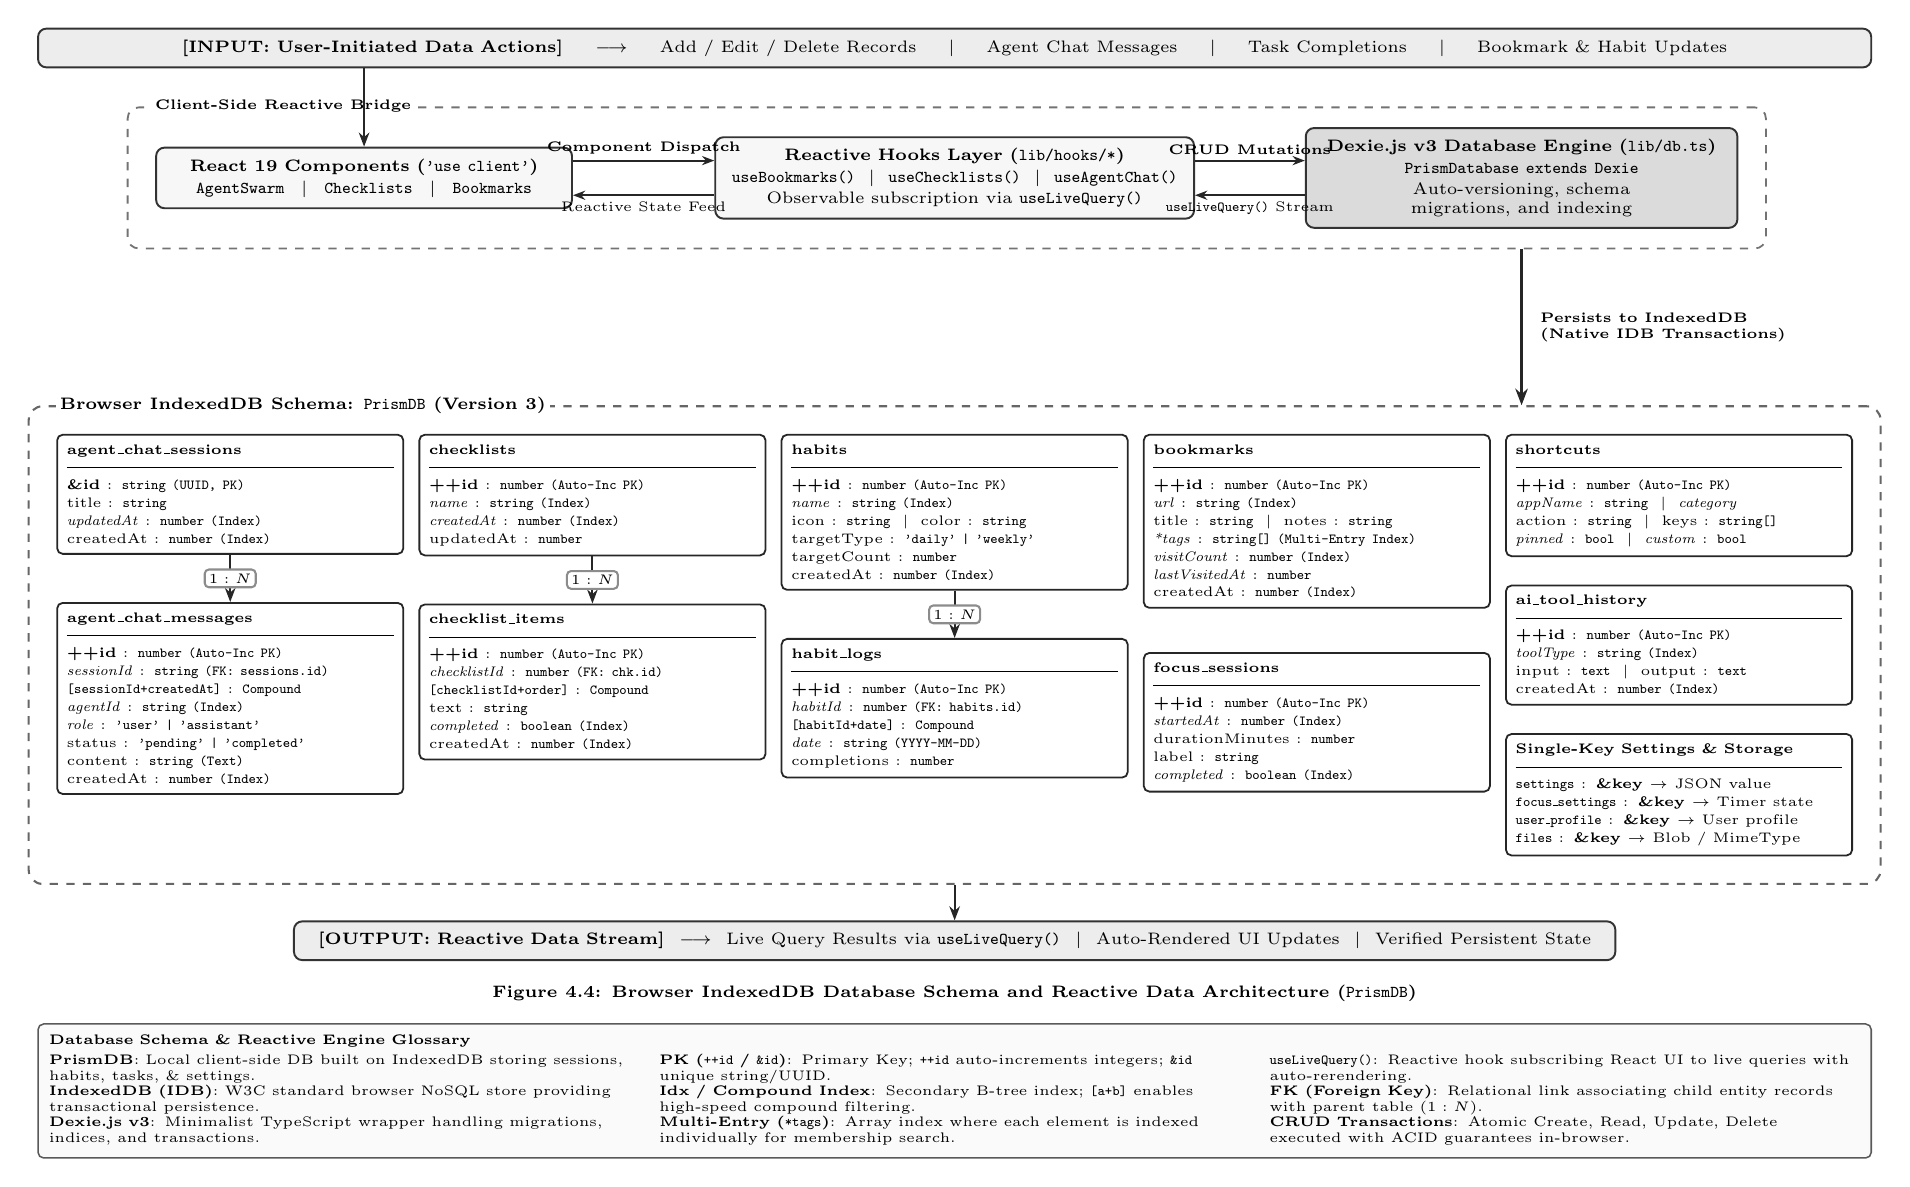
\begin{tikzpicture}[
    x=1cm, y=1cm,
    font=\sffamily,
    table/.style={
        rectangle,
        draw=black!85,
        line width=0.65pt,
        fill=white,
        rounded corners=2pt,
        text width=4.15cm,
        inner sep=3.5pt,
        font=\fontsize{5.4}{6.5}\selectfont
    },
    system_box/.style={
        rectangle,
        draw=black!80,
        line width=0.7pt,
        fill=black!3,
        rounded corners=3pt,
        inner sep=4pt,
        align=center,
        font=\fontsize{5.6}{6.8}\selectfont
    },
    rel_arrow/.style={
        -{Stealth[scale=0.8]},
        line width=0.75pt,
        draw=black!85
    }
]

    % =========================================================================
    % 1. TOP: INPUT NODE
    % =========================================================================
    \node [system_box, text width=23.0cm, fill=black!7] (input_node) at (0, 7.4) {
        \textbf{[INPUT: User-Initiated Data Actions]} $\;\longrightarrow\;$
        Add / Edit / Delete Records $\;\vert\;$ Agent Chat Messages $\;\vert\;$ Task Completions $\;\vert\;$ Bookmark \& Habit Updates
    };

    % =========================================================================
    % 2. MIDDLE: CLIENT-SIDE REACTIVE BRIDGE
    % =========================================================================
    \node [system_box, text width=5.0cm] (react_ui) at (-7.5, 5.75) {
        \textbf{React 19 Components (\texttt{'use client'})}\\[0.15em]
        \texttt{AgentSwarm} $\;\vert\;$ \texttt{Checklists} $\;\vert\;$ \texttt{Bookmarks}
    };

    \node [system_box, text width=5.8cm] (hooks_layer) at (0, 5.75) {
        \textbf{Reactive Hooks Layer (\texttt{lib/hooks/*})}\\[0.15em]
        \texttt{useBookmarks()} $\;\vert\;$ \texttt{useChecklists()} $\;\vert\;$ \texttt{useAgentChat()}\\[0.12em]
        Observable subscription via \textbf{\texttt{useLiveQuery()}}
    };

    \node [system_box, text width=5.2cm, fill=black!14] (dexie_engine) at (7.2, 5.75) {
        \textbf{Dexie.js v3 Database Engine (\texttt{lib/db.ts})}\\[0.15em]
        \texttt{PrismDatabase extends Dexie}\\[0.12em]
        Auto-versioning, schema migrations, and indexing
    };

    % Dual Parallel Reactive Flow Arrows with clean, outward labels
    \draw [-{Stealth[scale=0.75]}, line width=0.65pt, draw=black!85] ($(react_ui.east)+(0, 0.22)$) -- 
        node[above, font=\fontsize{4.8}{5.8}\bfseries\selectfont, inner sep=2pt]{Component Dispatch} ($(hooks_layer.west)+(0, 0.22)$);
    \draw [{Stealth[scale=0.75]}-, line width=0.65pt, draw=black!85] ($(react_ui.east)+(0, -0.22)$) -- 
        node[below, font=\fontsize{4.5}{5.5}\selectfont, inner sep=2pt]{Reactive State Feed} ($(hooks_layer.west)+(0, -0.22)$);
        
    \draw [-{Stealth[scale=0.75]}, line width=0.65pt, draw=black!85] ($(hooks_layer.east)+(0, 0.22)$) -- 
        node[above, font=\fontsize{4.8}{5.8}\bfseries\selectfont, inner sep=2pt]{CRUD Mutations} ($(dexie_engine.west)+(0, 0.22)$);
    \draw [{Stealth[scale=0.75]}-, line width=0.65pt, draw=black!85] ($(hooks_layer.east)+(0, -0.22)$) -- 
        node[below, font=\fontsize{4.5}{5.5}\selectfont, inner sep=2pt]{\textbf{\texttt{useLiveQuery()}} Stream} ($(dexie_engine.west)+(0, -0.22)$);

    % Bridge Container Boundary
    \node [draw=black!55, dashed, rounded corners=4pt, line width=0.65pt, 
           fit=(react_ui) (hooks_layer) (dexie_engine), inner xsep=0.35cm, inner ysep=0.25cm] (top_boundary) {};
    \node [anchor=west, font=\fontsize{5.4}{6.4}\bfseries\selectfont, fill=white, inner sep=1.5pt] at ($(top_boundary.north west)+(0.3,0)$) {Client-Side Reactive Bridge};

    % Arrow from INPUT down to React UI
    \draw [rel_arrow] (input_node.south -| react_ui.north) -- (react_ui.north);

    % =========================================================================
    % 3. DATABASE SCHEMA TABLES (5 COLUMNS) - ALIGNED AT NORTH y=2.5
    % =========================================================================

    % --- COLUMN 1: AGENT CHAT ---
    \node [table, anchor=north] (t_sessions) at (-9.2, 2.5) {
        \textbf{agent\_chat\_sessions}\\[-0.2em]
        \rule{\linewidth}{0.35pt}\\[0.15em]
        \pk{\&id} : \texttt{string (UUID, PK)}\\
        title : \texttt{string}\\
        \idx{updatedAt} : \texttt{number (Index)}\\
        createdAt : \texttt{number (Index)}
    };

    \node [table, below=0.6cm of t_sessions] (t_messages) {
        \textbf{agent\_chat\_messages}\\[-0.2em]
        \rule{\linewidth}{0.35pt}\\[0.15em]
        \pk{++id} : \texttt{number (Auto-Inc PK)}\\
        \idx{sessionId} : \texttt{string (FK: sessions.id)}\\
        \comp{[sessionId+createdAt]} : \texttt{Compound}\\
        \idx{agentId} : \texttt{string (Index)}\\
        \idx{role} : \texttt{'user' | 'assistant'}\\
        status : \texttt{'pending' | 'completed'}\\
        content : \texttt{string (Text)}\\
        createdAt : \texttt{number (Index)}
    };

    \draw [rel_arrow] (t_sessions.south) -- 
        node[draw=black!45, fill=white, rounded corners=1.5pt, inner sep=1.5pt, font=\fontsize{4.6}{5.6}\bfseries\selectfont]{$1 : N$} (t_messages.north);

    % --- COLUMN 2: CHECKLISTS ---
    \node [table, anchor=north] (t_checklists) at (-4.6, 2.5) {
        \textbf{checklists}\\[-0.2em]
        \rule{\linewidth}{0.35pt}\\[0.15em]
        \pk{++id} : \texttt{number (Auto-Inc PK)}\\
        \idx{name} : \texttt{string (Index)}\\
        \idx{createdAt} : \texttt{number (Index)}\\
        updatedAt : \texttt{number}
    };

    \node [table, below=0.6cm of t_checklists] (t_items) {
        \textbf{checklist\_items}\\[-0.2em]
        \rule{\linewidth}{0.35pt}\\[0.15em]
        \pk{++id} : \texttt{number (Auto-Inc PK)}\\
        \idx{checklistId} : \texttt{number (FK: chk.id)}\\
        \comp{[checklistId+order]} : \texttt{Compound}\\
        text : \texttt{string}\\
        \idx{completed} : \texttt{boolean (Index)}\\
        createdAt : \texttt{number (Index)}
    };

    \draw [rel_arrow] (t_checklists.south) -- 
        node[draw=black!45, fill=white, rounded corners=1.5pt, inner sep=1.5pt, font=\fontsize{4.6}{5.6}\bfseries\selectfont]{$1 : N$} (t_items.north);

    % --- COLUMN 3: HABITS ---
    \node [table, anchor=north] (t_habits) at (0.0, 2.5) {
        \textbf{habits}\\[-0.2em]
        \rule{\linewidth}{0.35pt}\\[0.15em]
        \pk{++id} : \texttt{number (Auto-Inc PK)}\\
        \idx{name} : \texttt{string (Index)}\\
        icon : \texttt{string} $\;\vert\;$ color : \texttt{string}\\
        targetType : \texttt{'daily' | 'weekly'}\\
        targetCount : \texttt{number}\\
        createdAt : \texttt{number (Index)}
    };

    \node [table, below=0.6cm of t_habits] (t_habit_logs) {
        \textbf{habit\_logs}\\[-0.2em]
        \rule{\linewidth}{0.35pt}\\[0.15em]
        \pk{++id} : \texttt{number (Auto-Inc PK)}\\
        \idx{habitId} : \texttt{number (FK: habits.id)}\\
        \comp{[habitId+date]} : \texttt{Compound}\\
        \idx{date} : \texttt{string (YYYY-MM-DD)}\\
        completions : \texttt{number}
    };

    \draw [rel_arrow] (t_habits.south) -- 
        node[draw=black!45, fill=white, rounded corners=1.5pt, inner sep=1.5pt, font=\fontsize{4.6}{5.6}\bfseries\selectfont]{$1 : N$} (t_habit_logs.north);

    % --- COLUMN 4: BOOKMARKS & FOCUS ---
    \node [table, anchor=north] (t_bookmarks) at (4.6, 2.5) {
        \textbf{bookmarks}\\[-0.2em]
        \rule{\linewidth}{0.35pt}\\[0.15em]
        \pk{++id} : \texttt{number (Auto-Inc PK)}\\
        \idx{url} : \texttt{string (Index)}\\
        title : \texttt{string} $\;\vert\;$ notes : \texttt{string}\\
        \idx{*tags} : \texttt{string[] (Multi-Entry Index)}\\
        \idx{visitCount} : \texttt{number (Index)}\\
        \idx{lastVisitedAt} : \texttt{number}\\
        createdAt : \texttt{number (Index)}
    };

    \node [table, below=0.55cm of t_bookmarks] (t_focus) {
        \textbf{focus\_sessions}\\[-0.2em]
        \rule{\linewidth}{0.35pt}\\[0.15em]
        \pk{++id} : \texttt{number (Auto-Inc PK)}\\
        \idx{startedAt} : \texttt{number (Index)}\\
        durationMinutes : \texttt{number}\\
        label : \texttt{string}\\
        \idx{completed} : \texttt{boolean (Index)}
    };

    % --- COLUMN 5: SHORTCUTS, TOOLS & SETTINGS ---
    \node [table, anchor=north] (t_shortcuts) at (9.2, 2.5) {
        \textbf{shortcuts}\\[-0.2em]
        \rule{\linewidth}{0.35pt}\\[0.15em]
        \pk{++id} : \texttt{number (Auto-Inc PK)}\\
        \idx{appName} : \texttt{string} $\;\vert\;$ \idx{category}\\
        action : \texttt{string} $\;\vert\;$ keys : \texttt{string[]}\\
        \idx{pinned} : \texttt{bool} $\;\vert\;$ \idx{custom} : \texttt{bool}
    };

    \node [table, below=0.35cm of t_shortcuts] (t_ai_tool) {
        \textbf{ai\_tool\_history}\\[-0.2em]
        \rule{\linewidth}{0.35pt}\\[0.15em]
        \pk{++id} : \texttt{number (Auto-Inc PK)}\\
        \idx{toolType} : \texttt{string (Index)}\\
        input : \texttt{text} $\;\vert\;$ output : \texttt{text}\\
        createdAt : \texttt{number (Index)}
    };

    \node [table, below=0.35cm of t_ai_tool] (t_kv) {
        \textbf{Single-Key Settings \& Storage}\\[-0.2em]
        \rule{\linewidth}{0.35pt}\\[0.15em]
        \texttt{settings} : \pk{\&key} $\rightarrow$ JSON value\\
        \texttt{focus\_settings} : \pk{\&key} $\rightarrow$ Timer state\\
        \texttt{user\_profile} : \pk{\&key} $\rightarrow$ User profile\\
        \texttt{files} : \pk{\&key} $\rightarrow$ Blob / MimeType
    };

    % Schema Container Boundary
    \node [draw=black!60, dashed, rounded corners=5pt, line width=0.75pt, 
           fit=(t_sessions) (t_messages) (t_checklists) (t_items) (t_habits) (t_habit_logs) (t_bookmarks) (t_focus) (t_shortcuts) (t_ai_tool) (t_kv), 
           inner xsep=0.35cm, inner ysep=0.35cm] (schema_boundary) {};
    \node [anchor=west, font=\fontsize{5.8}{7.0}\bfseries\selectfont, fill=white, inner sep=1.5pt] at ($(schema_boundary.north west)+(0.35,0)$) {Browser IndexedDB Schema: \texttt{PrismDB} (Version 3)};

    % Persistence Arrow connecting Dexie down into Schema
    \coordinate (persist_start) at (top_boundary.south -| dexie_engine.south);
    \coordinate (persist_end) at (schema_boundary.north -| dexie_engine.south);
    \draw [rel_arrow, line width=1.0pt] (persist_start) -- 
        node[right, font=\fontsize{5.0}{6.0}\bfseries\selectfont, align=left, xshift=3pt]{Persists to IndexedDB\\\fontsize{4.0}{5.0}\selectfont(Native IDB Transactions)} (persist_end);

    % =========================================================================
    % 4. BOTTOM: OUTPUT NODE
    % =========================================================================
    \node [system_box, text width=16.5cm, fill=black!7, below=0.45cm of schema_boundary] (output_node) {
        \textbf{[OUTPUT: Reactive Data Stream]} $\;\longrightarrow\;$
        Live Query Results via \texttt{useLiveQuery()} $\;\vert\;$ Auto-Rendered UI Updates $\;\vert\;$ Verified Persistent State
    };
    \draw [rel_arrow] (schema_boundary.south) -- (output_node.north);

    % Caption
    \node [font=\fontsize{6.0}{7.2}\bfseries\selectfont, below=0.18cm of output_node] (diag_caption) {
        Figure 4.4: Browser IndexedDB Database Schema and Reactive Data Architecture (\texttt{PrismDB})
    };

    % =========================================================================
    % 5. GLOSSARY TABLE
    % =========================================================================
    \node [rectangle, draw=black!65, line width=0.55pt, fill=black!2, rounded corners=2pt, 
           below=0.15cm of diag_caption, text width=23.0cm, inner sep=4pt, font=\fontsize{4.6}{5.6}\selectfont] (glossary_box) {
        \textbf{\fontsize{5.2}{6.2}\selectfont Database Schema \& Reactive Engine Glossary}\\[0.2em]
        \begin{tabular}{@{}>{\raggedright\arraybackslash}p{7.4cm}@{\hspace{0.35cm}}>{\raggedright\arraybackslash}p{7.4cm}@{\hspace{0.35cm}}>{\raggedright\arraybackslash}p{7.4cm}@{}}
        \textbf{PrismDB}: Local client-side DB built on IndexedDB storing sessions, habits, tasks, \& settings. &
        \textbf{PK (\texttt{++id} / \texttt{\&id})}: Primary Key; \texttt{++id} auto-increments integers; \texttt{\&id} unique string/UUID. &
        \textbf{\texttt{useLiveQuery()}}: Reactive hook subscribing React UI to live queries with auto-rerendering.\\
        \textbf{IndexedDB (IDB)}: W3C standard browser NoSQL store providing transactional persistence. &
        \textbf{Idx / Compound Index}: Secondary B-tree index; \texttt{[a+b]} enables high-speed compound filtering. &
        \textbf{FK (Foreign Key)}: Relational link associating child entity records with parent table ($1:N$).\\
        \textbf{Dexie.js v3}: Minimalist TypeScript wrapper handling migrations, indices, and transactions. &
        \textbf{Multi-Entry (\texttt{*tags})}: Array index where each element is indexed individually for membership search. &
        \textbf{CRUD Transactions}: Atomic Create, Read, Update, Delete executed with ACID guarantees in-browser.
        \end{tabular}
    };

\end{tikzpicture}%
}
\end{frame}

\end{document}
